\documentclass{article}
\usepackage[utf8]{inputenc}
\usepackage{graphicx}

\title{Approfondimenti EA}
\author{Cecca Francesco Pio}
\date{October 2021}

\begin{document}

\maketitle

\section{Rettificatori}

\textbf{Perchè quando sono accesi D1 e D3, D2 e D4 sono spenti? } \\
Perchè la tensione su D2 e D4 sarebbe negativa, di conseguenza per un diodo ideale si avrà un circuito aperto. \\ \\
\textbf{Perchè devo aggiungere un low-pass per migliorare le prestazioni del mio rettificatore?} \\
Perchè voglio produrre una tensione più continua possibile (con l'onda raddrizzata ci sono ancora troppe oscillazioni) \\ \\
\textbf{Come funziona un raddrizzatore con filtro?} \\
Supponiamo il condensatore inizialmente scarico (tensione ai suoi capi nulla). Il condensatore si carica durante la semionda positiva dell'onda di ingresso (quando il diodo è polarizzato direttamente). La sua carica (e dunque la tensione ai suoi capi) raggiunge il valore massimo in corrispondenza del massimo dell'onda. \\
Quando la tensione del generatore comincia a scendere, il condensatore "vorrebbe" scaricarsi. Tuttavia non può scaricarsi attraverso il diodo, poiché quest'ultimo impedisce il passaggio della corrente in quella direzione. In pratica il diodo si trova a essere polarizzato con una tensione sul catodo maggiore di quella presente sull'anodo: entra dunque in polarizzazione inversa. \\
Ciò ha l'effetto di "isolare" il gruppo RC dal resto del circuito: durante la semionda negativa, il condensatore si scarica sulla resistenza R. Il tempo di scarica dipende dal valore della costante di tempo del gruppo RC (tau = RC) e l'andamento della scarica è il tipico esponenziale decrescente. \\
Il diodo ricomincia a condurre (torna in polarizzazione diretta), solo quando la tensione del generatore supera la tensione sul condensatore. A questo punto il condensatore torna nuovamente a caricarsi fino al valore massimo e il processo si ripete allo stesso modo nei periodi successivi. \\
L'effetto finale è quello di produrre una tensione che, pur non essendo ancora "continua", ha oscillazioni molto minori dell'onda raddrizzata di partenza. In generale le ondulazione residue (dette ripple) sono tanto minori quanto maggiore è il valore della costante di tempo tau = RC del gruppo RC.

\section{Amplificatori Differenziali}

\textbf{Come ottengo gli specchi di corrente?} \\
Una corrente di riferimento di ingresso è applicata al BJT collegato come diodo, determinando una tensione base-emettitore (VBE1) adeguata a IB1.
\begin{center}
    Ir={Vcc-Vbe/R}
\end{center} 
La tensione di base-emettitore (VBE2) del transistor TR2 viene forzata ad uguagliare VBE1.
\begin{center}
    Ir={Ib1+Ib2+Ic1}  
\end{center}
Supponendo i due transistors identici, da VBE1 = VBE2 ne discende che IB1 = IB2 e IC1 = IC2 = I2, e tenendo presente la relazione in zona di funzionamento lineare fra correnti di base e di collettore IB = IC/b , i ha: 
\begin{equation}
    Ir=2Ib+Ic2=Ic2+2\cdot\frac{Ic2}{\beta} = \frac{\beta + 2}{\beta}\cdot Ic2 
\end{equation}
Dalla quale ricaviamo 
\begin{equation}
    Ic2\equiv{\frac{\beta}{\beta+2}\cdot Ir} \Rightarrow \beta >> 2 \Rightarrow Ic2={Ir}
\end{equation} \\
\textbf{PROBLEMA: Range di tensione} \\
Dipende, nel caso di specchi a MOSFET, dalla condizione che i 2 transistor siano in saturazione.
\begin{equation}
    v \geq v_{ds_{sat}}
\end{equation}
Quindi se la v cresce o scende, passa dalla saturazione al triodo/sottosoglia e quindi cambia la formula della corrente. Di conseguenza lo specchio non specchia più. \\ 
Per capire meglio analizzare la figura a pagina 3 \\ \\
\textbf{PROBLEMA: I deve essere più costante possibile al variare di v }\\
Questo perchè la R{o} è la R di Norton del generatore di corrente.
Se voglio usarlo in un amplificatore differenziale, R{o}  deve essere la più grande possibile affinchè il rumore diminuisca 

\subsection{Amplificatori Differenziali con Carico Attivo}
Gli specchi di corrente possono essere usati nell'amplificatore differenziale, oltre che per implementare il generatore di correrne di polarizzazione, anche per sostituire le R.\\
Dato che $i_{C_{3}}=i_{C_{4}}$ e $i_{c_{1}}=-i_{c_{2}}$ in AC
$i_{0}=i_{c_{4}}-i_{c_{2}}=i_{c_{3}}+i_{c_{1}}\simeq2i_{c_{1}}=g_{m}v_{d}$ \\
\begin{center}
    $2i_{c_{1}}=g_{m}v_{d}$  e  $\frac{v_{o}}{v_{d}}=g_{m}R_{L}$
\end{center}

\begin{center}
    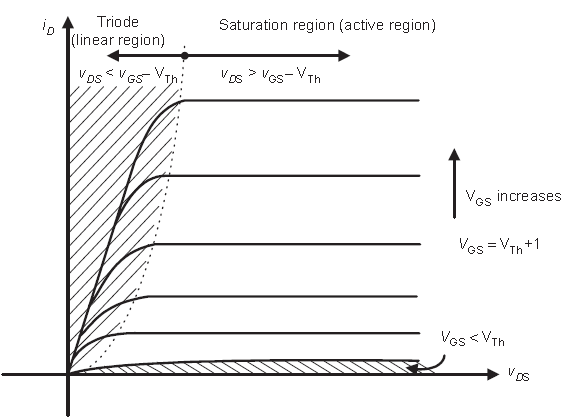
\includegraphics{image.png}
\end{center}

\newpage

\section{Comportamento in Frequenza}

\textbf{Metodo delle costanti di tempo}\\
Il metodo delle costanti di tempo a circuito aperto si usa per il calcolo dei coefficienti $b_{i}$ delle f.d.r così fatte:
\begin{equation}
    H(s)=\frac{1}{1+b_{1}s+b_{2}s^2+...+b_{n}s^n}
\end{equation}
Questa è una funzione LOW PASS, senza zeri o a frequenze così alte da essere trascurati.\\
Isolo i C in modo da rimanere con una rete A composta da elementi senza memoria.\\
Pongo il $det[Y]=0$ in modo da ottenere le frequenze naturali (poli del circuito).
\begin{equation}
    det[Y]=1+\sum b_{i}s^i
\end{equation}
Si è dimostrato che :
\begin{equation}
    b_{i}=\sum R_{i}C_{i} = \sum \tau_{i} => \omega_{H}=\frac{1}{b_{i}}=\frac{1}{\sum \tau_{i}}
\end{equation}
Per applicare il metodo delle costanti di tempo la $H_{H}$ deve essere scritta come la H(s) di sopra.\\
Quindi i condensatori che introducono uno zero prima del polo non vanno aggiunti nel metodo delle c.d.t per la stima della $\omega_{H}$\\
Per decidere si usa un generatore di test: se una volta cortocircuitato il C in esame, il guadagno diminuisce, allora il C va aggiunto, mentre se aumenta, non va considerato.\\
Viceversa per il metodo delle costanti di tempo a corto circuito.\\\\
\textbf{Quali condensatori usare?} \\
Analizzo prima quali condensatori usare per il \textbf{metodo a circuito aperto}.\\
Considerare, alle medie frequenze, che tutti i boli e gli zeri alle basse frequenze hanno già fatto effetto, equivale a considerare che tutti i condensatori responsabili di questi poli e zeri come cortocircuiti. \\ Quindi, la rete che corrisponde alla $ H_{h} $ (che lavora ad alte frequenze), è un amplificatore in AC con tutti i C di blocco/bypass cortocircuitati e con in evidenza i condensatori parassiti, i quali lavorano ad alte frequenze. \\
Analizzo, ora, quali condensatori usare per il \textbf{metodo a cortocircuito}.\\
Per il calcolo della $ \omega_{L} $
so che devo lavorare a basse frequenze e quindi avrò l'opposto di prima.\\ Quindi avrò che agiranno i C di blocco/bypass, mentre i C parassiti saranno circuiti aperti.
\newpage
\noindent
\textbf{Qual è il problema dell'EC?} \\
Analizzando e confrontando le $ \tau $ delle 3 configurazioni, noto che nell'EC le $ \tau $ sono molto più grandi e questo è un problema perchè, dal metodo delle costanti di tempo, so che la frequenza di taglio è l'inverso della somma delle $ \tau.$ \\
Quindi, avere costanti di tempo grandi, comporta una frequenza di taglio superiore bassa e quindi una banda più stretta e questo è un problemone perchè avere una banda stretta può causare distorsione del segnale che transita attraverso l'amplificatore, se questo ha delle componenti dello spettro a frequenza maggiori della frequenza di taglio superiore. \\ \\
\textbf{Collettore Comune - Emettitore Comune}\\
Sostituisco la $R_{S}$ di EC con la R d'uscita del CC.
Posso stare tranquillo che $\tau$ addizionali non vanificheranno il vantaggio ottenuto dalla diminuzione della $R_{i}$, data la alta frequenza di taglio della configurazione.\\
Il guadagno totale di tensione sarà circa uguale al guadagno di EC $A_{v_{EC}}$  dato che il CC ha $A_{v}=1$ se caricato da una R molto alta.

\newpage
\section{Retroazione}

\textbf{Come realizzo una retroazione positiva?} \\
Basta collegare la retroazione sul più, invece che sul meno, e questo comporterà il cambio si segno di $
    A(\omega)\beta $ \\ \\
\textbf{Analizzo la stabilità} \\
Per 1/2 poli è sempre verificata, mentre per 3 no perchè posso avere poli a Re>0 \\
Studio la stabilità con il criterio di Nyquist \\
\begin{equation}
    N=Z-P
\end{equation}
dove N è il numero di giri attorno a (-1,0), Z è il numero di zeri a Re>0 e P è il numero di poli a $
    Re>0
$ (risulterà P=0 perchè voglio studiare la stabilità e quindi non voglio poli a $
    Re>0
$.\\
Quindi la condizione di stabilità diventa:
\begin{equation}
    Z=0 => N=0
\end{equation}
Dalla definizione di stabilità regolare, cioè con una sola intersezione con il semiasse negativo, posso passare a Bode con condizioni ricavate osservando Nyquist.
\begin{enumerate}
    \item $ |A\beta(\omega_{\pi})|<1 ,   \phi(\omega_{\pi})=-\pi $
    \item $|A\beta(\omega_{t})|=1 ,   |\phi(\omega_{t})|<\pi$
\end{enumerate}
Se voglio graficare solo $A(\omega)$ si ha:
\begin{enumerate}
    \item $ |A(\omega_{\pi})|<\frac{1}{|\beta|} $ quando $ \phi(\omega_{\pi})=-\pi$
    \item $|A(\omega_{t})|=\frac{1}{|\beta|} $  quando $ |\phi(\omega_{t})|<\pi$
\end{enumerate}
\vspace{4mm}
\begin{center}
    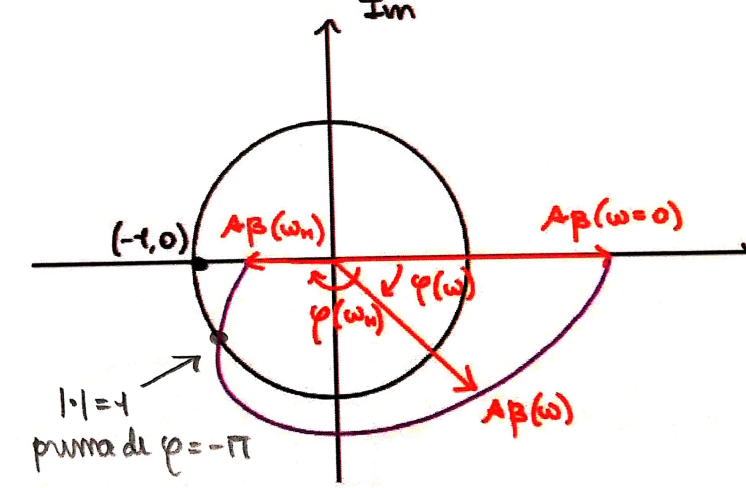
\includegraphics[scale=0.6]{Nyquist.png}
\end{center} 
\vspace{4mm}

\newpage
\noindent
Se $\frac{1}{\beta}=A_{F}$ fosse più basso, l'incrocio avverrebbe dopo. (vedi figura)
Quindi l'incrocio con $\frac{1}{\beta}$ deve avvenire prima di $\omega_{H}$ e per fare ciò potrei aver bisogno che $\frac{1}{\beta}=A_{F}$ sia molto alto. Se voglio un guadagno qualunque bisogna modificare l'amplificatore.
\begin{itemize}
    \item introduzione di un polo a low frequenza
    \item spostamento indietro del primo polo ottenuta aggiungendo una C a bassa frequenza
\end{itemize}
La seconda opzione, ovviamente è la migliore perchè aumenta la banda (1 decade in più) \\
\vspace{4mm}
\begin{center}
    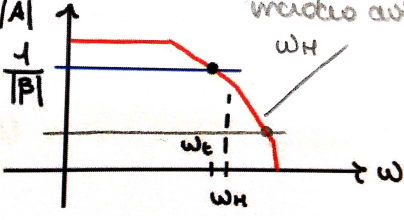
\includegraphics[scale=1]{Bode.png}
\end{center}
\vspace{4mm}
\subsection{ROC}
La stabilità può essere studiata con il margine di fase attraverso la \textbf{ROC}.
\begin{equation}
    \mbox {ROC = pendenza di} \frac{1}{\beta} - \mbox{pendenza di }A(\omega) 
\end{equation}
\begin{equation}
    \phi_{M}=180°-\frac{9}{2}ROC
\end{equation}

\newpage
\section{Amplificatori Operazionali}

\end{document}
